% 第 10 题四个极坐标图形选项，按固定来源第 1 页重绘。
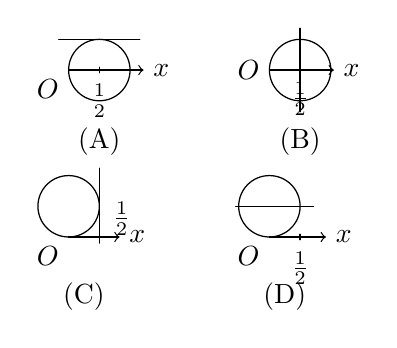
\begin{tikzpicture}[x=0.78cm,y=0.78cm,line width=0.45pt,line cap=round]
  % (A) rho=cos(theta) 对应圆心 (1/2,0)、半径 1/2；上方水平线相切。
  \begin{scope}
    \draw (0.5,0) circle (0.5);
    \draw (-0.16,0.5) -- (1.16,0.5);
    \draw[->] (0,0) -- (1.22,0) node[right] {$x$};
    \node[below left] at (0,0) {$O$};
    \draw (0.5,-0.045) -- (0.5,0.045);
    \node[below] at (0.5,-0.07) {$\frac12$};
    \node[below] at (0.5,-0.78) {(A)};
  \end{scope}

  % (B) 同一圆，x=1/2 直线通过圆心。
  \begin{scope}[xshift=2.55cm]
    \draw (0.5,0) circle (0.5);
    \draw (0.5,-0.68) -- (0.5,0.68);
    \draw[->] (0,0) -- (1.05,0) node[right] {$x$};
    \node[left] at (0,0) {$O$};
    \node[below] at (0.5,-0.04) {$\frac12$};
    \node[below] at (0.5,-0.78) {(B)};
  \end{scope}

  % (C) 干扰图：圆底端为 O，右侧竖线与圆相切。
  \begin{scope}[yshift=-2.12cm]
    \draw (0,0.5) circle (0.5);
    \draw (0.5,-0.10) -- (0.5,1.12);
    \draw[->] (0,0) -- (0.83,0) node[right] {$x$};
    \node[below left] at (0,0) {$O$};
    \node[right] at (0.56,0.30) {$\frac12$};
    \node[below] at (0.25,-0.58) {(C)};
  \end{scope}

  % (D) 干扰图：圆底端为 O，水平线通过圆心。
  \begin{scope}[xshift=2.55cm,yshift=-2.12cm]
    \draw (0,0.5) circle (0.5);
    \draw (-0.55,0.5) -- (0.72,0.5);
    \draw[->] (0,0) -- (0.92,0) node[right] {$x$};
    \node[below left] at (0,0) {$O$};
    \draw (0.5,-0.045) -- (0.5,0.045);
    \node[below] at (0.5,-0.08) {$\frac12$};
    \node[below] at (0.25,-0.58) {(D)};
  \end{scope}
\end{tikzpicture}
